% n90.tex

\section{Dissociating nitrogen flow over a 2D cylinder}
\label{sec:n90}
\index{chemical reaction!example of use}
\index{finite-rate chemistry|see {chemical reaction}}
\index{gas model!thermally perfect!example of use}
%
High speed flow of nitrogen over a 2D cylinder is a signature experiment for shock tunnel
and expansion tube facilities.
This example shows the construction of a simple flow domain around a circular cylinder
and the set up of a finite-rate reacting model for dissociating nitrogen.
The data for comparison has come from our colleagues at DLR-G\"{o}ttingen.

\begin{figure}[htbp]
\begin{center}
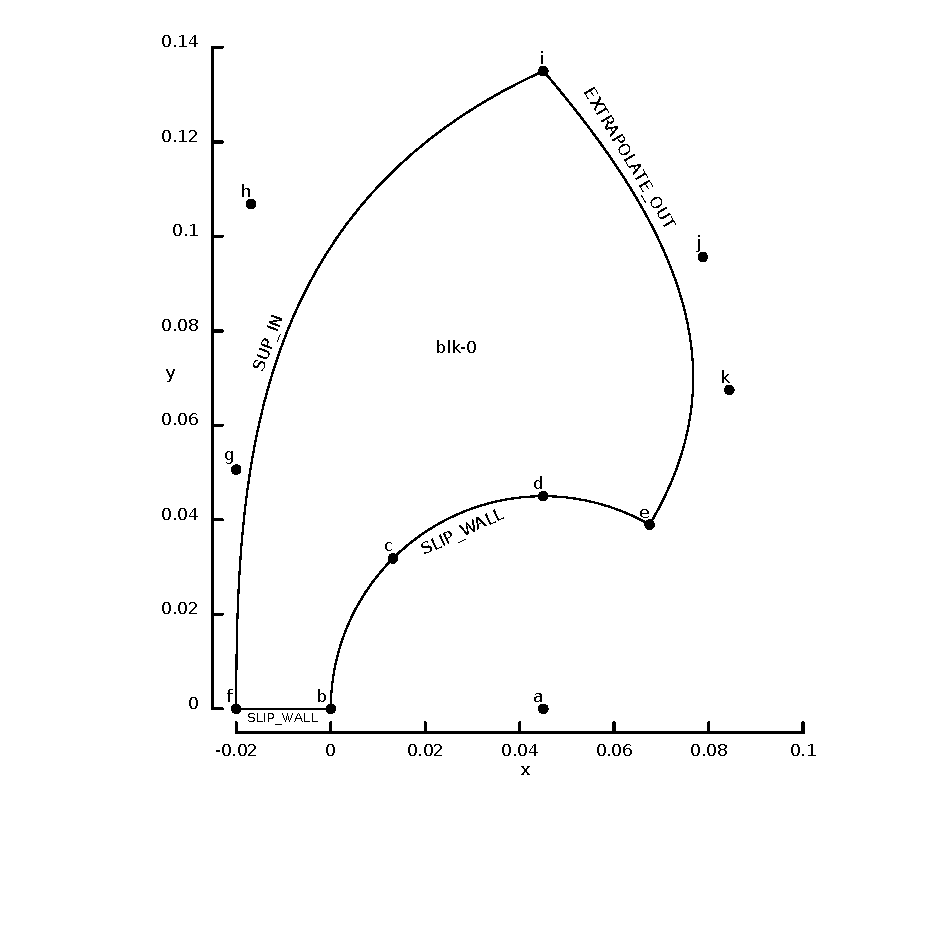
\includegraphics[width=12cm,viewport=76 80 391 439,clip=true]{../2D/n90/n90-schematic.pdf}
\end{center}
\caption{Schematic diagram of the geometry for the bluff body.}
\label{n90-geometry-fig}
\end{figure}

\begin{figure}[htbp]
\begin{center}
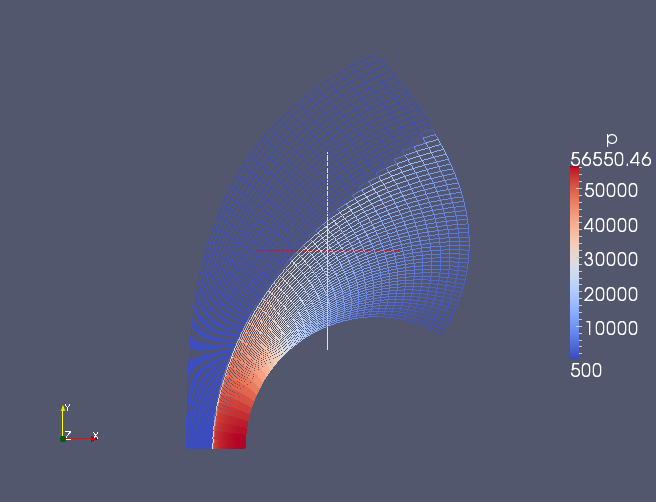
\includegraphics[width=\textwidth]{../2D/n90/n90-pressure-mesh.png}
\end{center}
\caption{Mesh, coloured by pressure, for the n90 bluff body exercise.}
\label{n90-mesh-fig}
\end{figure}

\begin{figure}[htbp]
\begin{center}
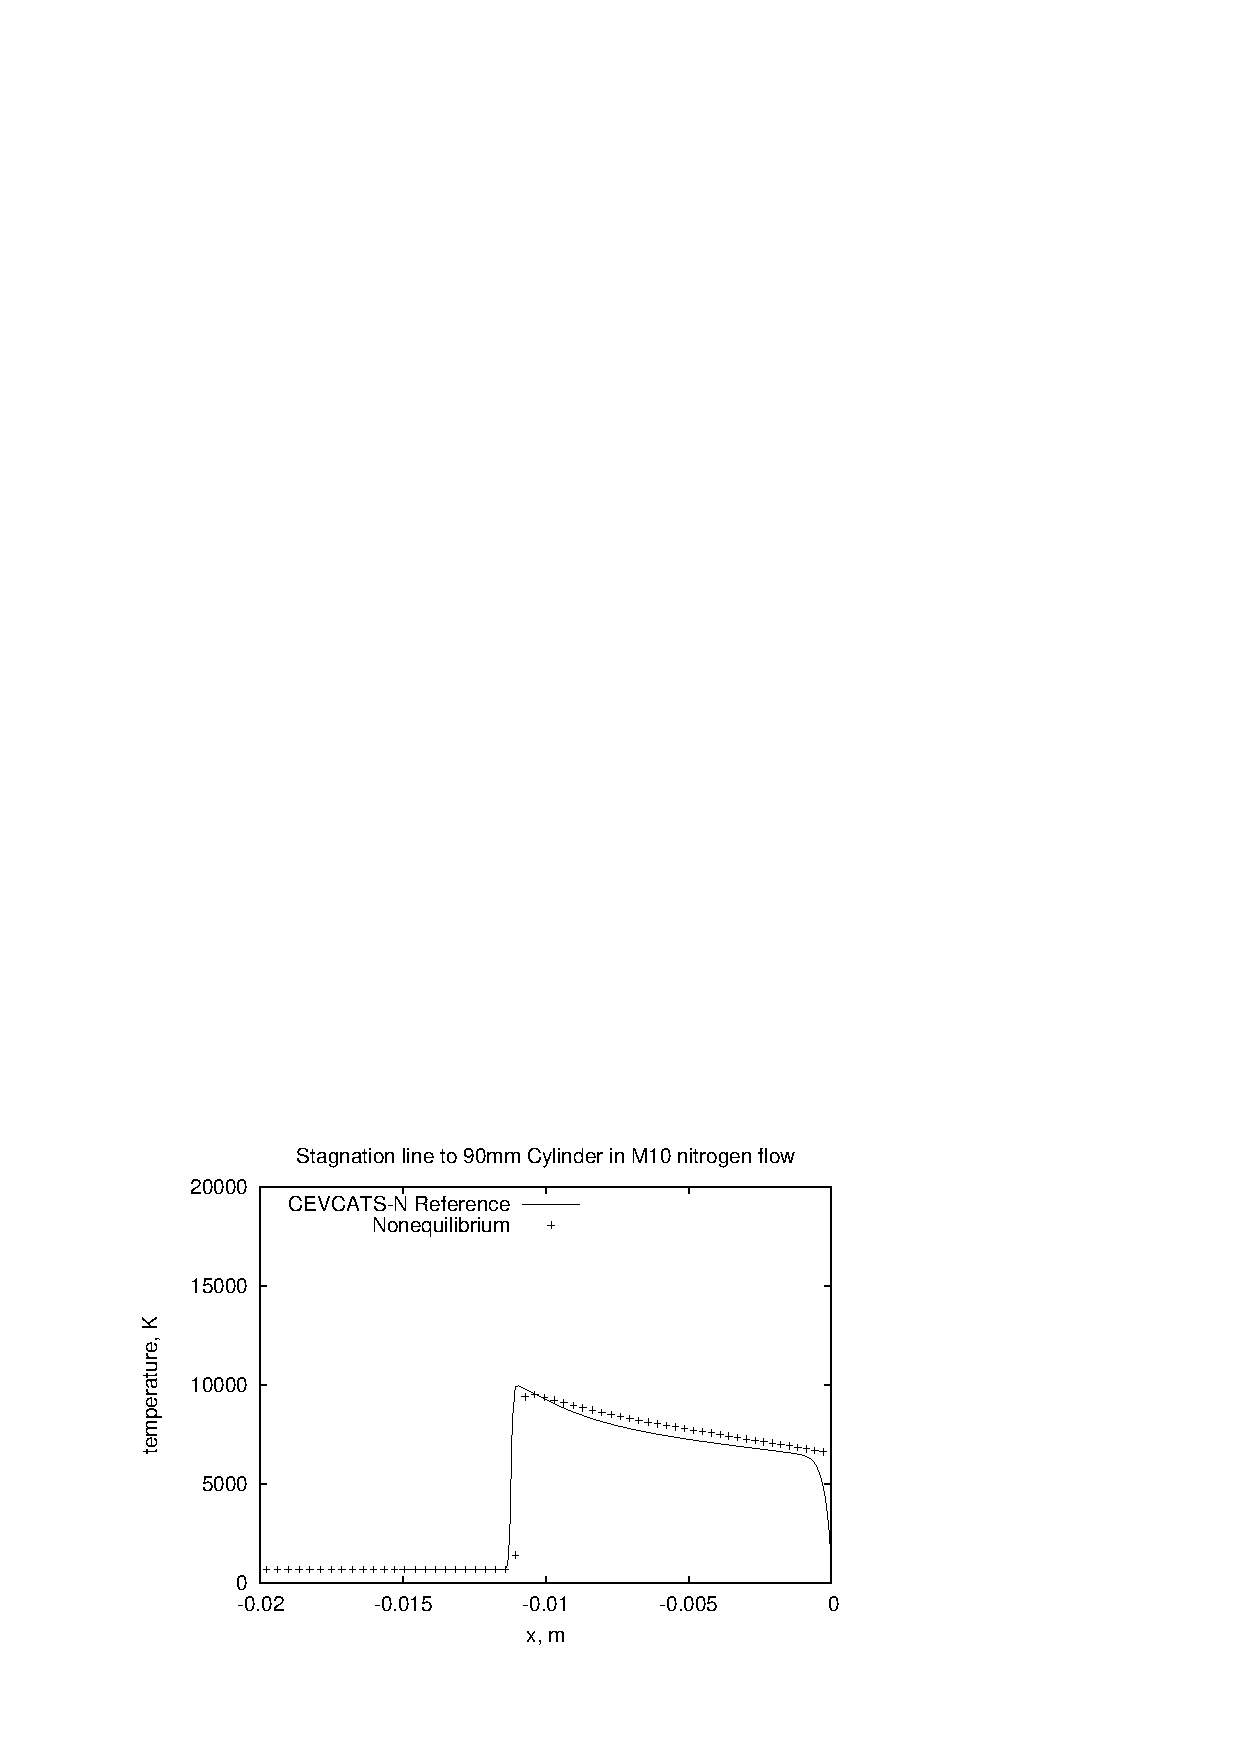
\includegraphics[width=12cm, viewport=67 53 403 291]{../2D/n90/n90_compare_T_stag_line.pdf}
\end{center}
\caption{Temperature data along the stagnation streamline.}
\label{n90-stag-line-temp-fig}
\end{figure}

\begin{figure}[htbp]
\begin{center}
\mbox{
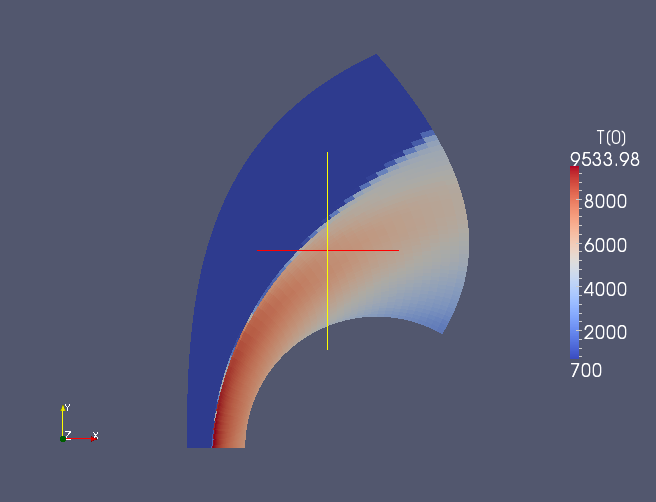
\includegraphics[width=0.5\textwidth]{../2D/n90/n90-temperature.png}
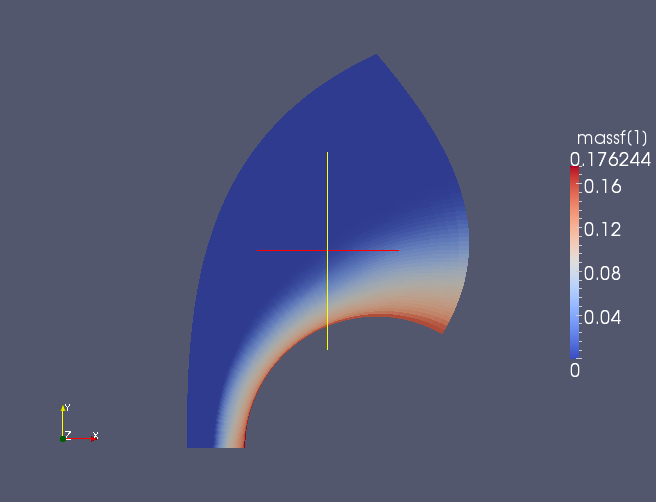
\includegraphics[width=0.5\textwidth]{../2D/n90/n90-massf1.png}
}
\end{center}
\caption{Temperature and mass fraction of nitrogen atoms for the n90 bluff body exercise.}
\label{n90-temperature-massf-fig}
\end{figure}

\newpage

\subsection{Input script (.py)}
\topbar
\lstinputlisting[language={}]{../2D/n90/n90.py}
\bottombar

\subsection{Reaction scheme file (.lua)}\index{chemical reaction!reaction scheme file!dissociating nitrogen}
\topbar
\lstinputlisting[language={}]{../2D/n90/nitrogen-2sp-2r.lua}
\bottombar

\subsection{Shell scripts}
\label{n90-sh-files}
\topbar
\lstinputlisting[language={}]{../2D/n90/prepare_simulation.sh}
\bottombar

\noindent
\topbar
\lstinputlisting[language={}]{../2D/n90/run_simulation.sh}
\bottombar

\noindent
\topbar
\lstinputlisting[language={}]{../2D/n90/post_simulation.sh}
\bottombar

\noindent
\topbar
\lstinputlisting[language={}]{../2D/n90/plot_comparison.gnu}
\bottombar

\subsection{Notes}
\begin{itemize}
\item For Eilmer3, this simulation required 9\,min, 21\,sec on a single core of 
  a Pentium 1.6\,GHz processor to reach a final time of 100$\mu$s in 3406 steps.
\end{itemize}
